The Camassa-Holm equation was studied first by Camassa and Holm \cite{camassa1993integrable} and is defined as

\begin{align*}
u_{t} - u_{xxt} + 2\kappa u_{x} + 3uu_{x} - 2u_{x}u_{xx} - uu_{xxx} = 0,
\end{align*}

or (if $\kappa = 0$) equivalently in the Hamiltonian form

\begin{align}
m &= u - u_{xx} \notag \\
m_t &= -2mu_x - um_x.
\label{eq:CHhamiltonian}
\end{align}

The equation is used to model waves in shallow water. The characteristic solutions of this equation are solitary waves of permanent shape, traveling at constant speed. If these waves can interact with other waves of the same type without changing their shape or speed, they are called solitons. 



In this paper, the only cases considered are when $\kappa = 0$. This is sufficient due to the fact that solutions for a nonzero $\kappa$ are obtained from the solutions using $\kappa = 0$ by the transformation $v(x,t) = u(x + \kappa t, t) - \kappa$. Removing this term makes the soliton solutions peaked. These solutions are called peakons and have a discontinuity in the first derivative in the peak. Peakons also have a constant traveling speed equal to its height.

A single peakon is presented in figure \ref{fig:peakon} and we see that the peakon retains its shape over time. Any linear combination of peakons is called a multipeakon, one can be seen in figure \ref{fig:doublepeakon}. Peakons can also interact with other peakons of different size, and in figure \ref{fig:peakonovertake} we see that both of the peakons retain their original form after the collision is over. Finally we see in figure \ref{fig:peakonantipeakon} a peakon and an antipeakon collide. An antipeakon is a negative peakon. What is shown here is the solution that conserves the energy. Another solution would be the zero line to eternity (non-conservative solution).

\begin{figure}[h]
        \centering
        \begin{subfigure}[b]{0.49\textwidth}
                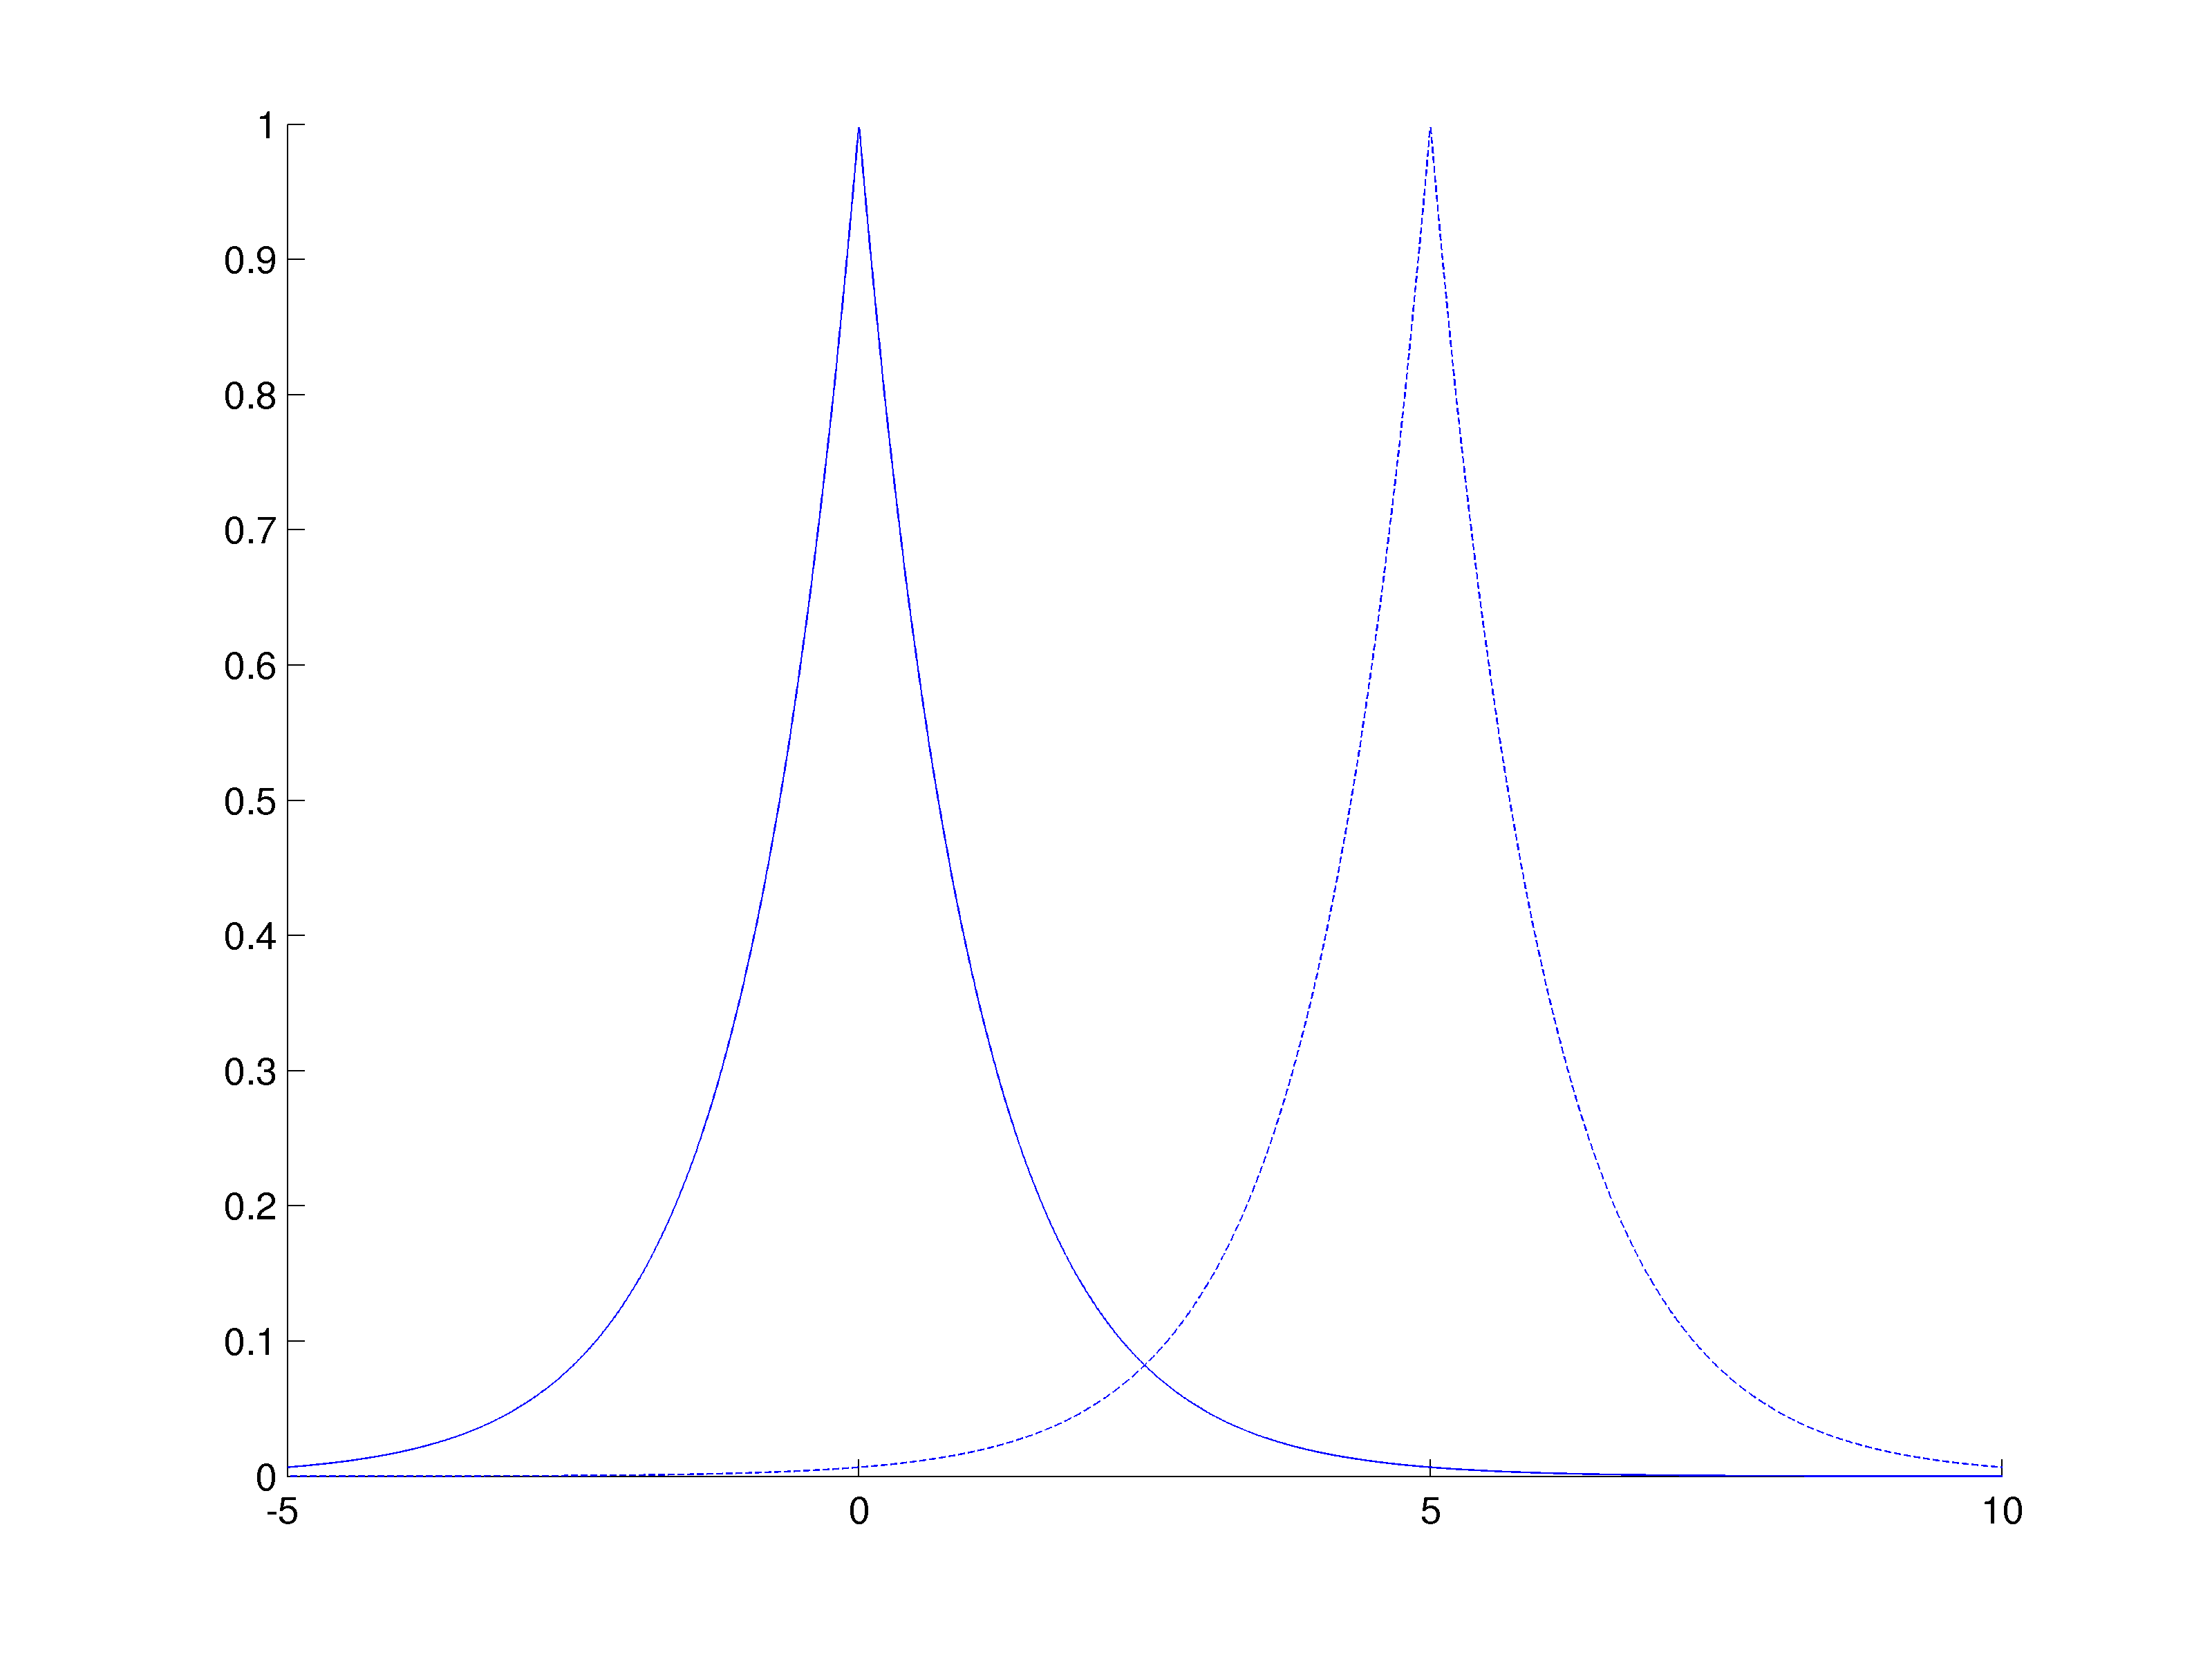
\includegraphics[width=\textwidth]{gfx/peakon}
                \caption{A peakon, t = [0, 5].}
                \label{fig:peakon}
        \end{subfigure}
        \begin{subfigure}[b]{0.49\textwidth}
                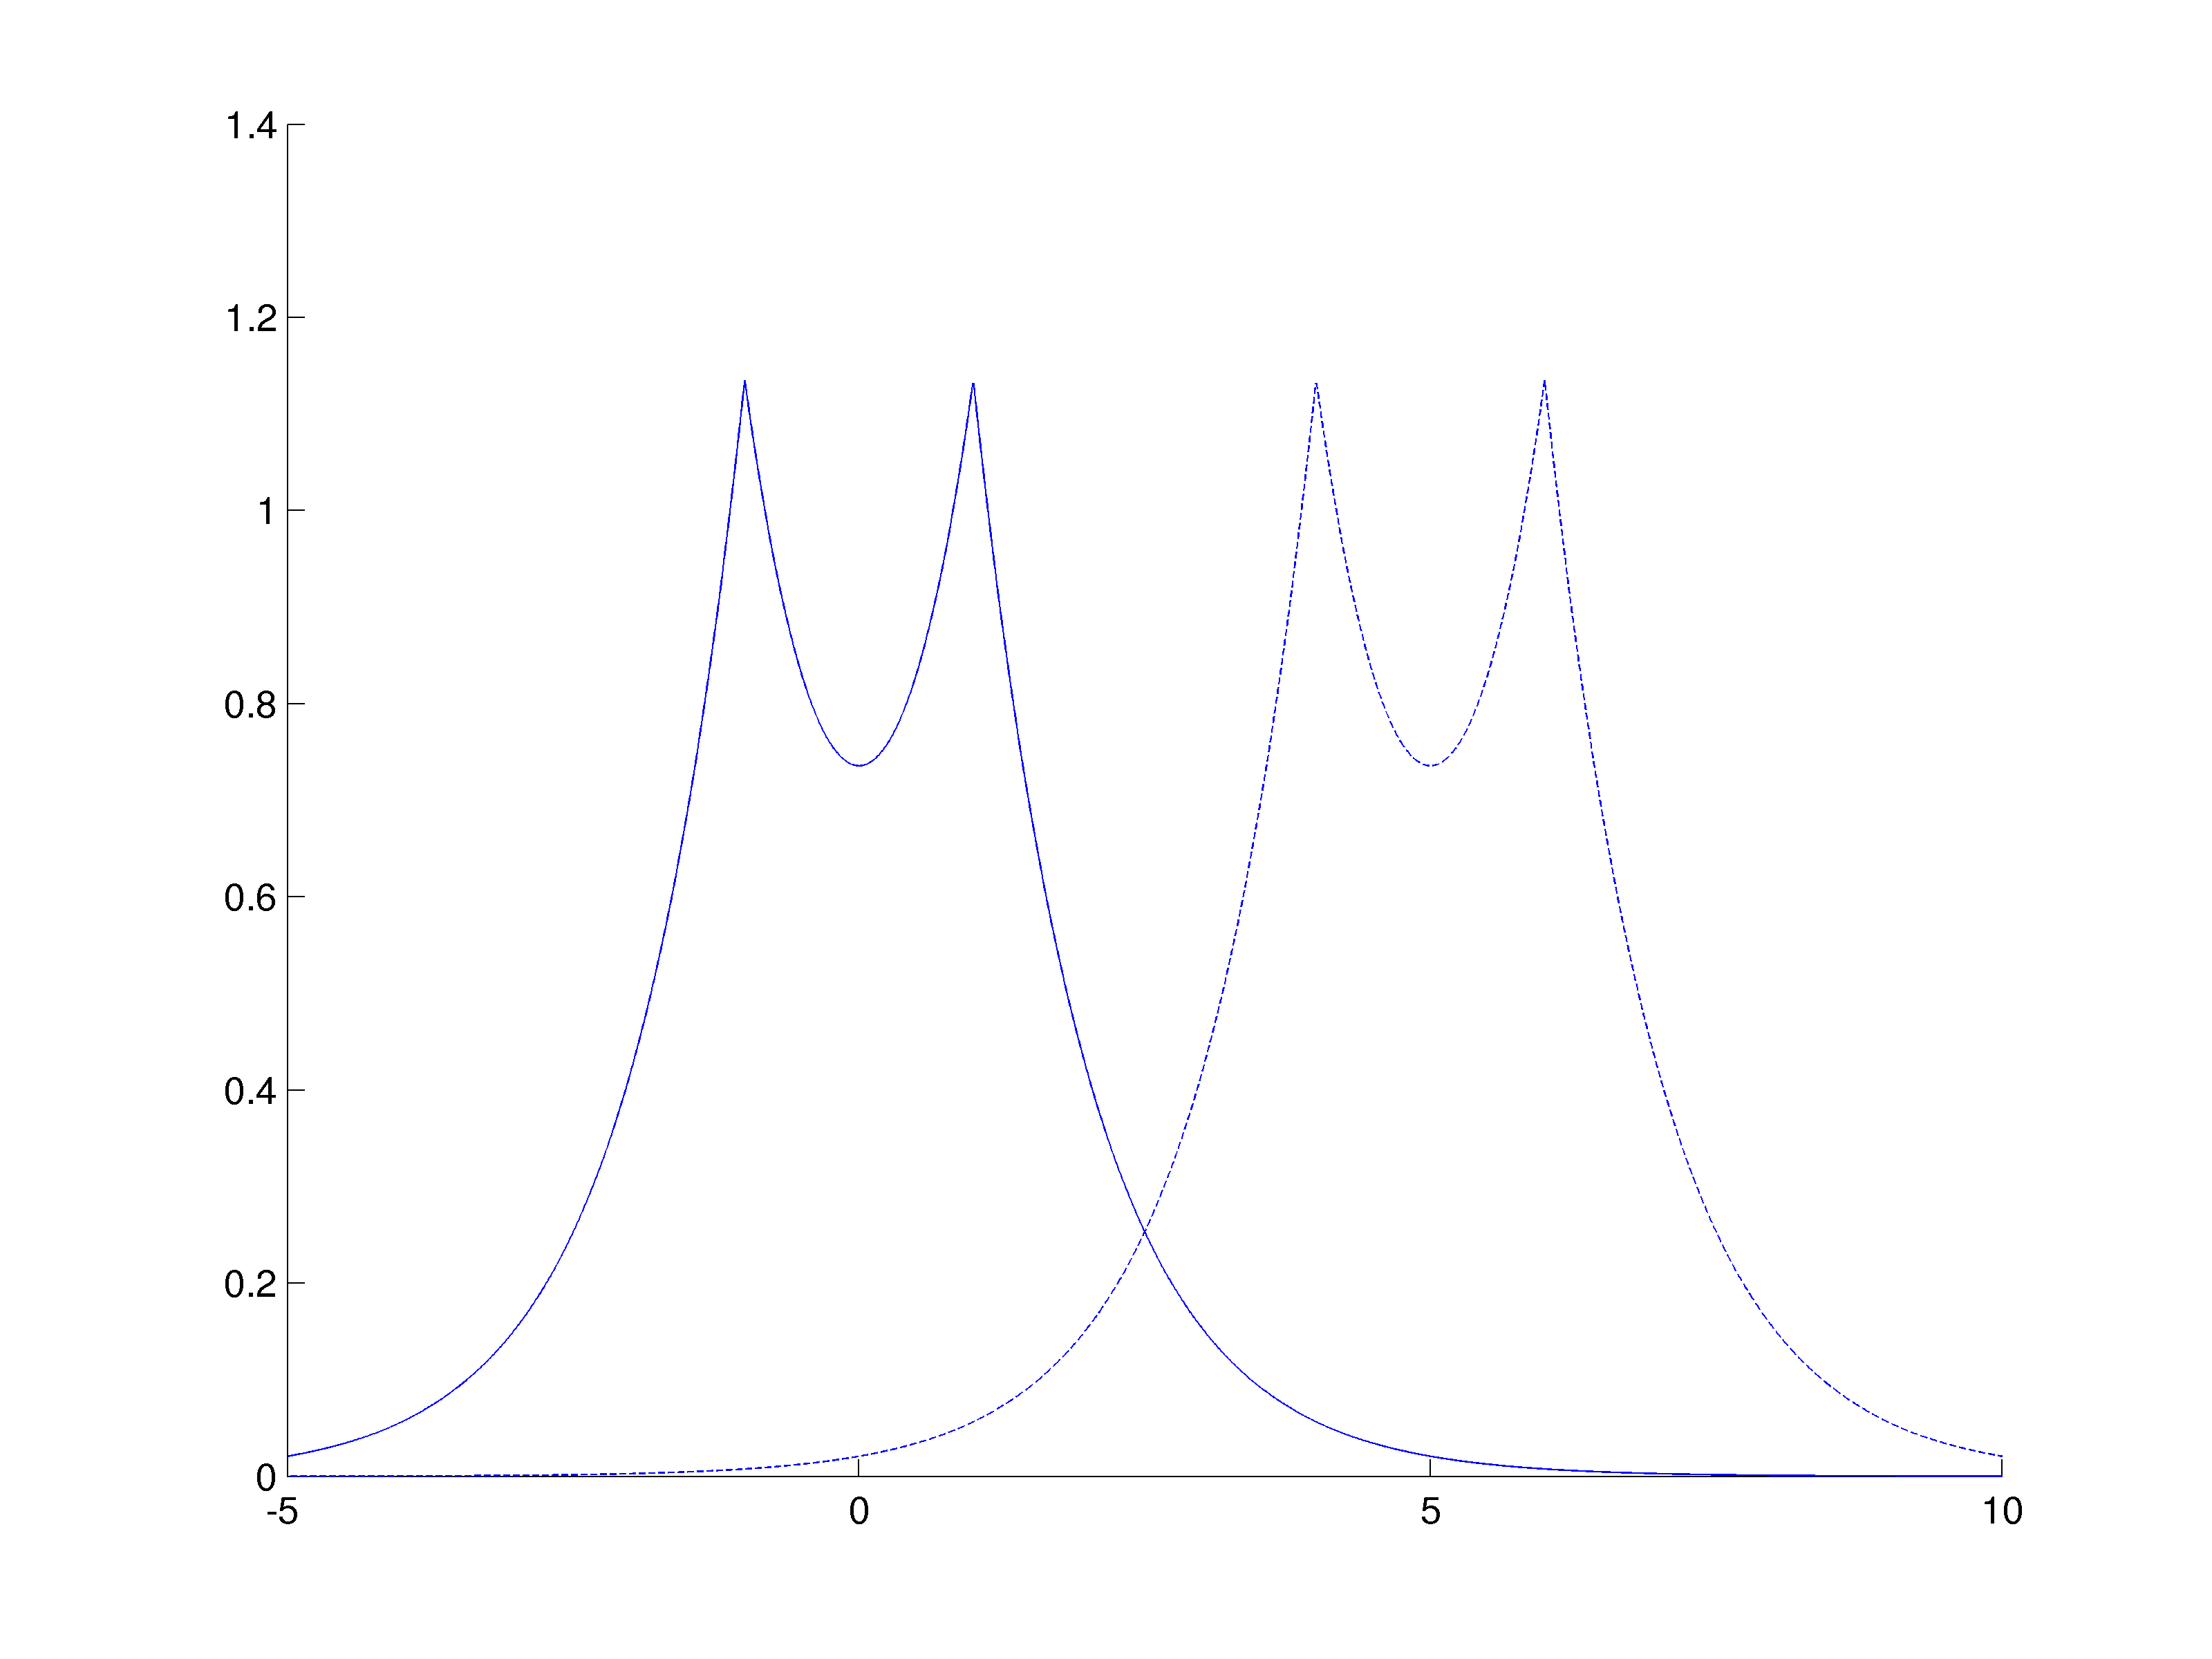
\includegraphics[width=\textwidth]{gfx/doublepeakon}
                \caption{A doublepeakon, t = [0, 5].}
                \label{fig:doublepeakon}
        \end{subfigure}
        \begin{subfigure}[b]{0.49\textwidth}
                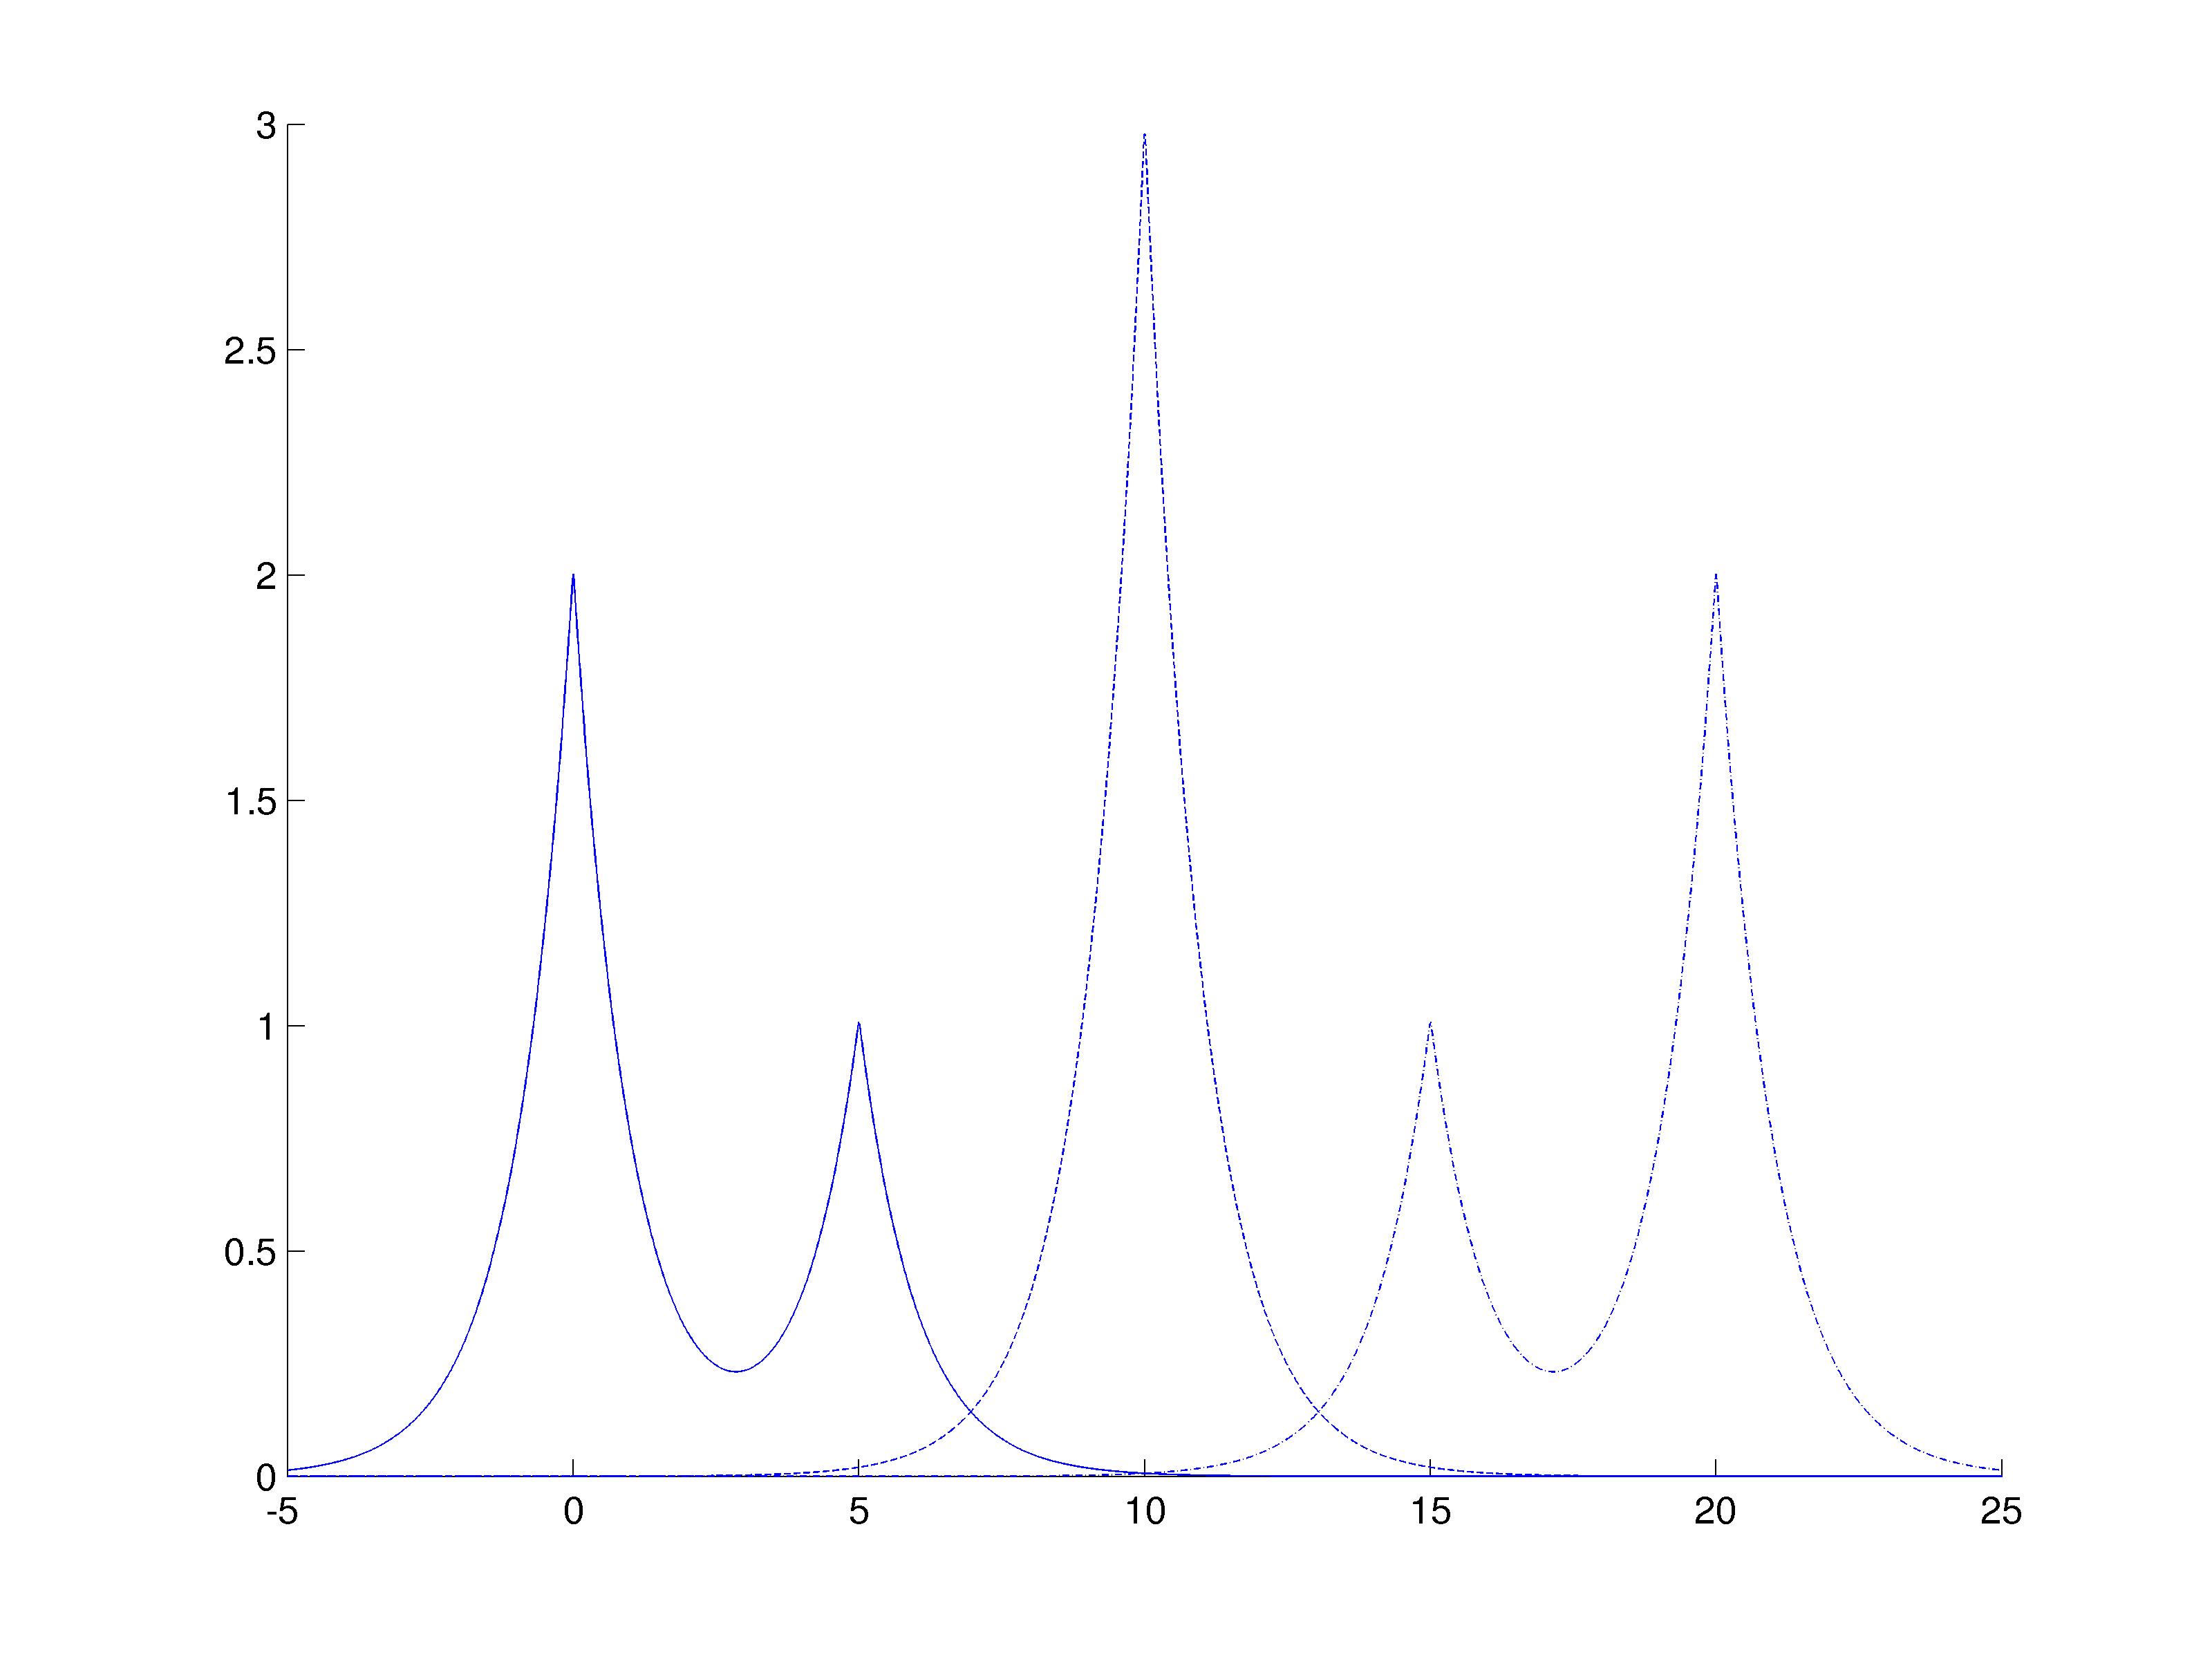
\includegraphics[width=\textwidth]{gfx/peakonovertake}
                \caption{Two peakons collide, t = [0, 5, 10]}
                \label{fig:peakonovertake}
        \end{subfigure}
        \begin{subfigure}[b]{0.49\textwidth}
                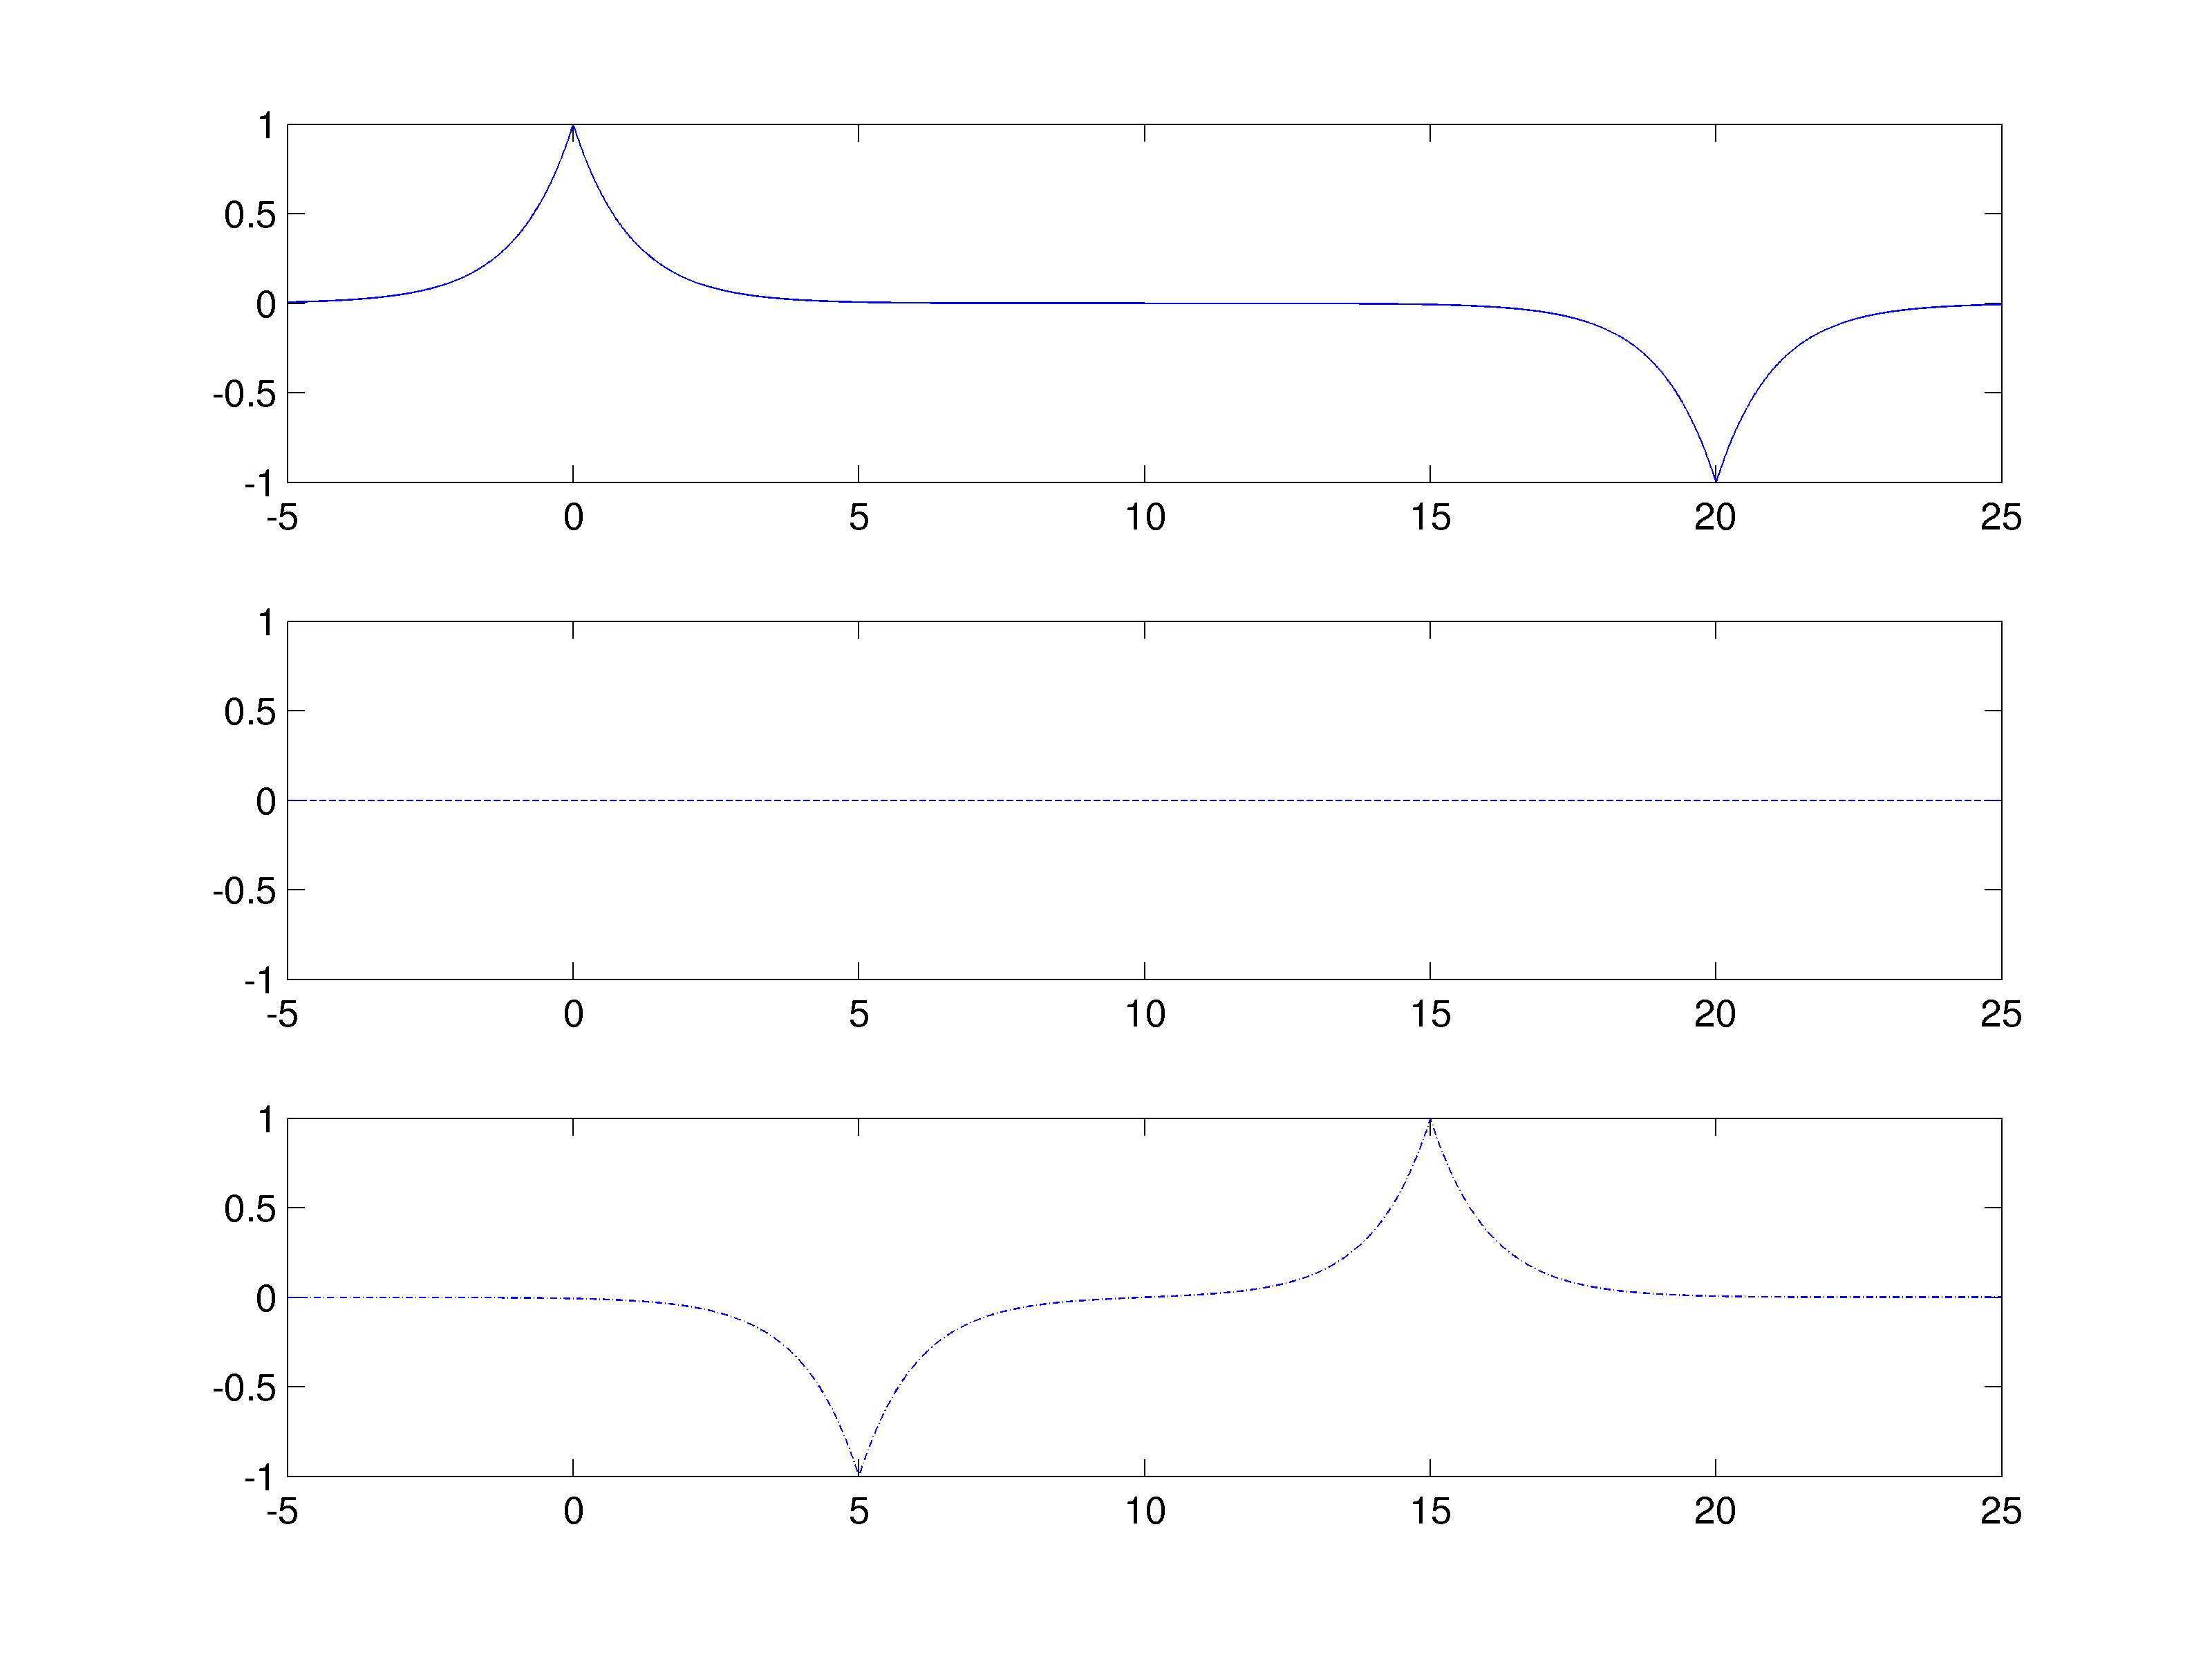
\includegraphics[width=\textwidth]{gfx/peakonantipeakon}
                \caption{Peakon - antipeakon, [t = 0, 10, 15]}
                \label{fig:peakonantipeakon}
        \end{subfigure}
        \caption{Interactions between peakons.}
\end{figure}

Following we define a finite difference scheme to solve the Camassa-Holm equation. Our scheme is highly influenced by a scheme found by Holden and Raynaud \cite{holden2006convergence}.
